\documentclass[12pt]{article}
    \usepackage[margin=1in]{geometry}
    \usepackage{mdframed}
    \usepackage{subcaption}
    \usepackage{amssymb}
    \usepackage{amsmath}
    \usepackage{mathtools}
    \usepackage{centernot}
    \usepackage[ruled,vlined,linesnumbered]{algorithm2e}
    \definecolor{lapislazuli}{rgb}{0.15, 0.38, 0.61}
    \newcommand{\CommentFont}[1]{\texttt{\color{lapislazuli}#1}}
    \SetCommentSty{CommentFont}
    \SetKwComment{Comment}{// }{}
    % Custom colors
    \usepackage{color}
    \definecolor{deepblue}{rgb}{0,0,0.5}
    \definecolor{deepred}{rgb}{0.6,0,0}
    \definecolor{deepgreen}{rgb}{0,0.5,0}
    % Default fixed font does not support bold face
    \DeclareFixedFont{\ttb}{T1}{txtt}{bx}{n}{12} % for bold
    \DeclareFixedFont{\ttm}{T1}{txtt}{m}{n}{12}  % for normal
    \usepackage{listings}
    \usepackage{url}

    \usepackage{booktabs}
    \usepackage{hyperref}

    \usepackage{tikz}
    \usetikzlibrary{shapes,arrows,automata,positioning,cd}
    \tikzset{
      cfgedge/.style   = {black, ->, >=stealth},
      forward/.style = { blue, ->, >=angle 45},
      backward/.style = { red, densely dashed, ->, >=latex' },
      backwardleft/.style = { red, densely dashed, <-, >=latex' },
    }
    \usepackage{xcolor}

    \newcommand{\cfgarrow}{\mathbin{\tikz[baseline]\draw[cfgedge,yshift=0.6ex] (0,0) -- (.9em,0);}}
    \newcommand{\forwardarrow}{\mathbin{\tikz[baseline]\draw[forward,yshift=0.6ex] (0,0) -- (1em,0);}}
    \newcommand{\backwardarrow}{\mathbin{\tikz[baseline]\draw[backward,yshift=0.6ex] (0,0) -- (.95em,0);}}
    \newcommand{\dom}{\underline{\gg}}

    
    \begin{document}
    \lstset{
    language=C,
    basicstyle=\ttfamily\small,
    keywordstyle=\ttb\color{deepblue}\small,
    emph={foo,bar,assert,baz},          % Custom highlighting
    emphstyle=\ttb\color{deepred}\small,    % Custom highlighting style
    stringstyle=\color{deepgreen}\small,
    frame=tb,                         % Any extra options here
    showstringspaces=false            % 
    }
    
    \begin{center}
        \bigskip
        {\LARGE ECS 240 Programming Languages} \medskip
        
        {\Large Homework 1} \bigskip
    
    \end{center}
    
    \section*{About This Assignment}
    
    \begin{itemize}
      \item This assignment tests you on your understanding of dominators and
      control dependence.
      \item To complete the assignment (i)~modify \texttt{hw1.tex}, (ii)~create
      the corresponding PDF document (using pdflatex, for example), and
      (iii)~submit the pdf electronically via Gradescope by the due date; see
      \href{https://www.gradescope.com/get_started#student-submission}{this page}
      and
      \href{http://gradescope-static-assets.s3-us-west-2.amazonaws.com/help/submitting_hw_guide.pdf}{this
      document}. Your assignment will not be graded and you will receive no
      points if you do not follow these instructions. 

      \item \textbf{When submitting the assignment on Gradescope, please mark
      which page corresponds to each question on the assignment.}  Your
      assignment will not be graded and you will receive no points if you do not
      mark the pages.      

      \item The  \LaTeX\ source has \texttt{TODO}~comments to clearly indicate
      where changes need to be made. 
      \item The \verb=\vspace= commands can be safely commented out.
      \item This assignment can be worked on in a group of at most three. Enter
      the names and email addresses of the team members in the space provided
      below.
    \end{itemize}

    \begin{mdframed}
      Team members:
      \begin{itemize}
        %TODO
        \item Divyansh Rajesh Jain, drajeshjain@ucdavis.edu % Enter name and email address of first team member.
        \item Soham Kolhatkar, sakolhatkar@ucdavis.edu % Comment out this line if working individually.
        % \item Name, email address % Comment out this line if working in pairs.
      \end{itemize}
    \end{mdframed}
    
    \newpage
    \begin{enumerate}

      
      \item Prove the following about the dominator relation $\dom$:
      \begin{enumerate}
        \item (5 points) If $a \dom b$ and $b \dom c$, then $a \dom c$
        (transitivity).
        \begin{mdframed}
          %\vspace{2em}
          %% TODO
          Suppose we assume that \( a \dom b \) and \( b \dom c \), but \( a \centernot{\dom} c \).

          \medskip

          That means that there is some path from the entry node to node \( c \) that does \emph{not} include node \( a \).

          \medskip

          We know that \( b \dom c \), which means that every path from the entry node to \( c \) must contain node \( b \).  
          This implies that node \( b \) is definitely on every path from the entry to \( c \).

          \medskip

          Therefore, the path from the entry to \( c \) that does not include \( a \) must still include node \( b \).  
          This means the problem has now shifted: there exists some path from the entry node to node \( b \) that does not include node \( a \).

          \medskip

          But this contradicts our original assumption that \( a \dom b \), which means that every path from the entry node to node \( b \) must contain node \( a \).  
          Hence, such a path cannot exist.

          \medskip

          Therefore, there cannot be any path from the entry node to node \( c \) that does not contain node \( a \).

          \medskip

          Thus, we have shown that if \( a \dom b \) and \( b \dom c \), then \( a \dom c \).

        \end{mdframed}

        \item (5 points) It is never possible that both $a \dom b$ and $b \dom
        a$, if $a \neq b$ (anti-symmetry).
        \begin{mdframed}
          %\vspace{2em}
          %% TODO
          Suppose that \( a \dom b \), \( b \dom a \), and \( a \neq b \).

          \medskip

          From \( a \dom b \), we know that every path from the entry node to node \( b \) includes node \( a \).  
          If we enumerate all paths from the entry node to the exit node that contain node \( b \) as sequences, node \( a \) must appear before node \( b \) in every possible sequence.

          \medskip

          Similarly, from \( b \dom a \), we know that every path from the entry node to node \( a \) includes node \( b \).  
          Therefore, If we enumerate all paths from the entry node to the exit node that contain node \( a \) as sequences, node \( b \) must appear before node \( a \) in every possible sequence.

          \medskip

          Putting these two facts together, for every path from the entry node to the exit node that contain either node \( a \) or node \( b \):

          \begin{enumerate}
              \item node \( a \) must appear before node \( b \).
              \item node \( b \) must appear before node \( a \).
          \end{enumerate}

          This is only possible if \( a = b \)

          \medskip

          But this contradicts our original assumption that \( a \neq b \).

          \medskip

          Therefore, we have shown that it is not possible for both \( a \dom b \) and \( b \dom a \) to hold if \( a \neq b \).

        \end{mdframed}

        \item (5 points) If $a$ and $b$ are two dominators of $n$, then either
        $a \dom b$ or $b \dom a$ must hold.
        \begin{mdframed}
          %\vspace{2em}
          %% TODO
          \textbf{Case 1: \( a = b \)}

          If \( a = b \), then the statement holds trivially, because a node dominates itself.  
          Therefore, \( a \dom b \) and \( b \dom a \).

          \medskip

          \textbf{Case 2: \( a = n \) or \( b = n \)}

          \begin{itemize}
              \item If \( a = n \), then the statement holds trivially because \( b \dom a \), since \( b \dom n \) and \( a = n \).
              \item If \( b = n \), then the statement holds trivially because \( a \dom b \), since \( a \dom n \) and \( b = n \).
          \end{itemize}

          \medskip

          \textbf{Case 3: \( a \) and \( b \) are strict dominators of \( n \), and \( a \neq b \)}

          Since both \( a \) and \( b \) dominate \( n \), every path from the entry node to node \( n \) must include both node \( a \) and node \( b \).
          This means that every path contains \( a \) and \( b \), but it is possible that \( a \) comes before \( b \) in some paths and vice versa. 
          This is the same thing as saying that $a \dom b$ and $b \dom a$.

          \medskip

          However, from our previous proof, we know that if \( a \neq b \), then it is impossible for both \( a \dom b \) and \( b \dom a \) to be true.

          \medskip

          Thus, it must be the case that either \( a \dom b \) or \( b \dom a \).

          \medskip

          Therefore, in all cases, $a \dom b$ or $b \dom a$ if $a \dom n$ and $b \dom n$.

        \end{mdframed}

        \item (5 points) Each node $n$ except the entry has a unique
        \emph{immediate dominator} --- the dominator that appears closest to $n$
        along any acyclic path from the entry to $n$.
        \begin{mdframed}
          Suppose there are $j$ nodes $a_1, \ldots, a_j$ such that $a_1 \dom n, \ldots, a_j \dom n$. That means that on every path from the entry node to node $n$, all of the nodes $a_1, \ldots, a_j$ must appear.

          \textbf{Case 1: One of the nodes $a_1, \ldots, a_j$ is a predecessor of $n$}

          Since this node is a dominator of $n$, every path from entry to $n$ must pass through it. Therefore, no other node can be the immediate dominator of $n$, because that would imply the existence of a path from entry to $n$ that skips this predecessor — contradicting the fact that it dominates $n$.

          Furthermore, only one of the nodes $a_1, \ldots, a_j$ can be a predecessor of $n$. If more than one were predecessors, then there would be a path from entry to $n$ that skips one of them, violating the assumption that each $a_i$ dominates $n$.

          \textbf{Case 2: None of the nodes $a_1, \ldots, a_j$ are predecessors of $n$}

          Let us pick two nodes $a_k$ and $a_z$ from the set $a_1, \ldots, a_j$. We know that both $a_k \dom n$ and $a_z \dom n$.

          Now suppose there exists a path where $a_k$ is the immediate dominator of $n$, and another path where $a_z$ is the immediate dominator of $n$.

          That would imply that:
          \begin{itemize}
            \item There is a path of the form:
            \[
            entry \rightarrow \cdots \rightarrow a_z \rightarrow \cdots \rightarrow a_k \rightarrow \cdots \rightarrow n
            \]
            such that $a_k$ is the immediate dominator of $n$. So there exists a path from $a_k$ to $n$ that does not pass through any other dominator (in particular, not through $a_z$).

            \item There is another path of the form:
            \[
            entry \rightarrow \cdots \rightarrow a_k \rightarrow \cdots \rightarrow a_z \rightarrow \cdots \rightarrow n
            \]
            such that $a_z$ is the immediate dominator of $n$, meaning there is a path from $a_z$ to $n$ that does not pass through any other dominator (specifically not through $a_k$).
          \end{itemize}

          But this creates a contradiction. If $a_z$ is the immediate dominator of $n$, then there exists a path from $a_z$ to $n$ that avoids $a_k$. So in the first path, we could replace the subpath from $a_z$ to $a_k$ with the shorter path that goes directly from $a_z$ to $n$ — skipping $a_k$. This would imply the existence of a path from entry to $n$ that skips $a_k$, which contradicts the assumption that $a_k \dom n$.

          The same contradiction arises if we assume $a_k$ is the immediate dominator. Therefore, both cannot be the immediate dominator of $n$.

          Since this argument applies to any distinct pair of nodes among $a_1, \ldots, a_j$, we conclude that there is a unique immediate dominator of $n$.
        \end{mdframed}
      \end{enumerate}


      \begin{figure}[h]
        \centering
        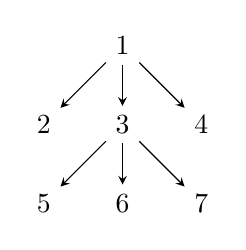
\begin{tikzpicture}[auto,node distance=1cm] 
        \node (1) {1};
        \node [below of=1] (3) {3};
        \node [left of=3] (2) {2};
        \node [right of=3] (4) {4};
        \node [below of=3] (6) {6};
        \node [left of=6] (5) {5};
        \node [right of=6] (7) {7};
        
        \path (1) edge[cfgedge] (2); 
        \path (1) edge[cfgedge] (3);
        \path (1) edge[cfgedge] (4);
        \path (3) edge[cfgedge] (5);
        \path (3) edge[cfgedge] (6);
        \path (3) edge [cfgedge](7);
        \end{tikzpicture}
        \caption{Dominator tree $T_1$}
        \label{fig:tree1}
      \end{figure}
      % 3
      \item (3 points) Consider the dominator tree $T_1$ in
      Figure~\ref{fig:tree1}. Draw \textbf{one} control-flow graph whose
      dominator tree is $T_1$. Recall that a control-flow graph (CFG) has a
      single entry node (a node with no incoming edges), a single exit node (a
      node with no outgoing edges), and all nodes are reachable from the entry
      node. 
      \begin{mdframed}
          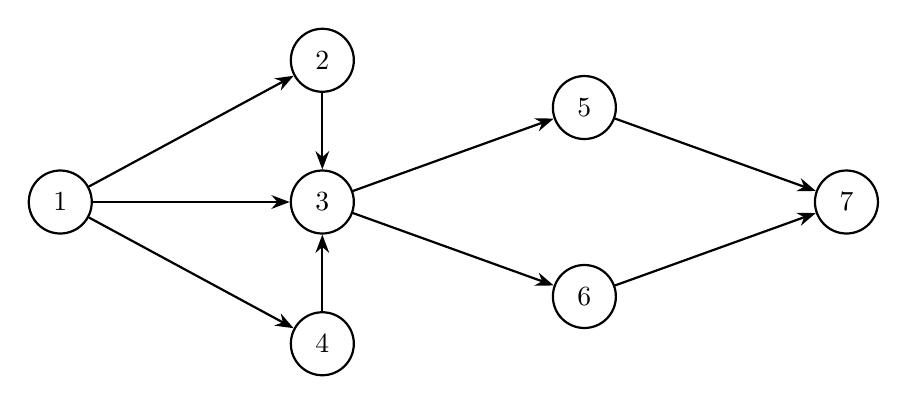
\begin{tikzpicture}[
            node distance=1.5cm and 2.5cm,
            every node/.style={circle, draw, minimum size=8mm},
            every path/.style={->, thick, >=Stealth}
          ]

          % Nodes
          \node (1) {1};
          \node[right=of 1, yshift=1.8cm] (2) {2};
          \node[right=of 1] (3) {3};
          \node[right=of 1, yshift=-1.8cm] (4) {4};
          \node[right=of 3, yshift=1.2cm] (5) {5};
          \node[right=of 3, yshift=-1.2cm] (6) {6};
          \node[right=of 5, yshift=-1.2cm] (7) {7};

          % Edges
          \draw (1) -- (2);
          \draw (1) -- (3);
          \draw (1) -- (4);
          \draw (2) -- (3);
          \draw (4) -- (3);
          \draw (3) -- (5);
          \draw (3) -- (6);
          \draw (5) -- (7);
          \draw (6) -- (7);

        \end{tikzpicture}
        %% TODO
      \end{mdframed}

      \clearpage
      \item (5 points) State whether the following statement is \textbf{True} or
      \textbf{False}: 

        \emph{Given a flow graph $G$, if there is an control-flow edge from node
        $u$ to node $v$, then the immediate dominator of $v$ dominates $u$.}

      If \textbf{True}, provide a proof.
      If \textbf{False}, provide a counter-example in the form of the flow graph
      $G$ and the nodes $u$~and~$v$.
      \begin{mdframed}
        \textbf{True} 

        \textbf{Proof:}

        Let the immediate dominator of node $v$ be node $d$. By definition, $d$ is the closest strict dominator of $v$ — that is, $d \dom v$, and no other node strictly between $d$ and $v$ on any path from the entry to $v$ also dominates $v$.

        Suppose, that $d$ does not dominate node $u$.

        Then there exists a path from the entry node to $u$ that does not pass through $d$. Since there is a control flow edge from $u$ to $v$, we can extend this path by adding the edge $(u, v)$, forming a new path from entry to $v$ that avoids $d$.

        But this contradicts the fact that $d$ dominates $v$, since we’ve found a path from entry to $v$ that does not go through $d$.

        Therefore, our assumption must be false. Hence, the immediate dominator $d$ of node $v$ must also dominate node $u$.
      \end{mdframed}

      \clearpage
      \begin{figure}[h]
        \centering
        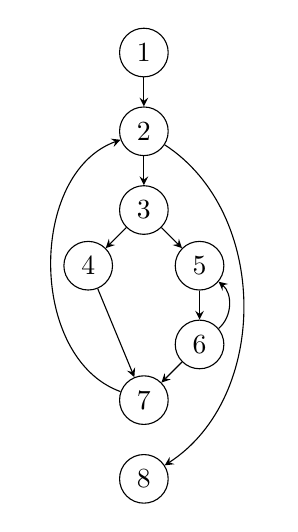
\begin{tikzpicture}[auto,node distance=1cm] 
        \tikzstyle{every node} = [circle, draw]
        \node (1) {1};
        \node [below of=1] (2) {2};
        \node [below of=2] (3) {3};
        \node [below left of=3] (4) {4};
        \node [below right of=3] (5) {5};
        \node [below of=5] (6) {6};
        \node [below left of=6] (7) {7};
        \node [below of=7] (8) {8};
        
        \path (1) edge[cfgedge] (2); 
        \path (2) edge [cfgedge,bend left=57] (8);
        \path (2) edge[cfgedge] (3);
        \path (3) edge[cfgedge] (4);
        \path (3) edge[cfgedge] (5);
        \path (4) edge[cfgedge] (7);
        \path (5) edge [cfgedge](6);
        \path (6) edge[cfgedge,bend right=50] (5);
        \path (6) edge[cfgedge] (7);
        \draw (7) edge [cfgedge, bend left=70] (2);
        \end{tikzpicture}
        \caption{Directed graph $G$}
        \label{fig:graph1}
      \end{figure}
      \item (10 points) The route of the search in a depth-first search of a
      directed graph forms a \emph{depth-first spanning tree (DFST)}. When we
      construct a DFST for a flow graph, the edges of the flow graph fall into
      three categories (i)~\emph{advancing edges}: edges that go from a node $m$
      to a proper descendent of $m$ in the tree, (ii)~\emph{retreating edges}:
      edges that go from a node $m$ to an ancestor of $m$ in the tree (possibly
      to $m$ itself), and (iii)~\emph{cross edges}: edges $m \cfgarrow n$ such
      that $m$ nor $n$ is an ancestor of the other in the DFST.

      The DFST representation of graph $G$ (Figure~\ref{fig:graph1}) is shown in
      Figure~\ref{fig:dfst1}. Advancing edges for indicated using $\cfgarrow$,
      retreating edges using $ \backwardarrow $, and cross edges using
      $\forwardarrow$.

      \begin{figure}[h]
        \centering
        \begin{subfigure}[b]{0.50\linewidth}
          \centering
            
          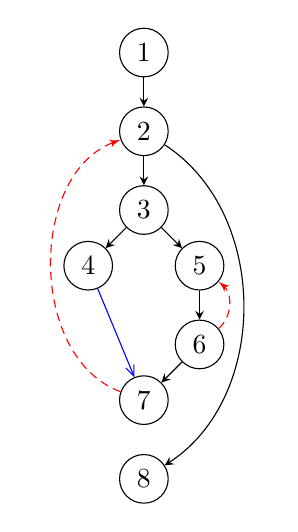
\begin{tikzpicture}[auto,node distance=1cm] 
          \tikzstyle{every node} = [circle, draw]
          \node (1) {1};
          \node [below of=1] (2) {2};
          \node [below of=2] (3) {3};
          \node [below left of=3] (4) {4};
          \node [below right of=3] (5) {5};
          \node [below of=5] (6) {6};
          \node [below left of=6] (7) {7};
          \node [below of=7] (8) {8};
          
          \path (1) edge[cfgedge] (2); 
          \path (2) edge [cfgedge,bend left=57] (8);
          \path (2) edge[cfgedge] (3);
          \path (3) edge[cfgedge] (4);
          \path (3) edge[cfgedge] (5);
          \path (4) edge[forward] (7);
          \path (5) edge [cfgedge](6);
          \path (6) edge[backward,bend right=50] (5);
          \path (6) edge[cfgedge] (7);
          \draw (7) edge [backward, bend left=70] (2);
          \end{tikzpicture}
        \caption{DFST representation of graph $G$ (Figure~\ref{fig:graph1}).}
        \label{fig:dfst1}
        \end{subfigure}
        %
        \begin{subfigure}[b]{0.40\linewidth}
          \centering
      
          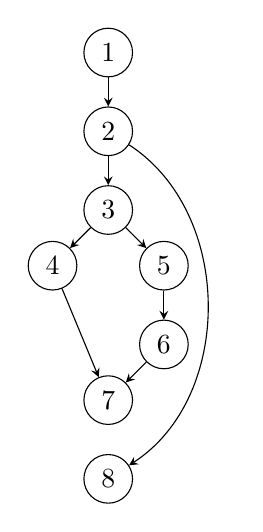
\begin{tikzpicture}[auto,node distance=1cm] 
          \tikzstyle{every node} = [circle, draw]
          \node (1) {1};
          \node [below of=1] (2) {2};
          \node [below of=2] (3) {3};
          \node [below left of=3] (4) {4};
          \node [below right of=3] (5) {5};
          \node [below of=5] (6) {6};
          \node [below left of=6] (7) {7};
          \node [below of=7] (8) {8};
          
          \path (1) edge[cfgedge] (2); 
          \path (2) edge [cfgedge,bend left=57] (8);
          \path (2) edge[cfgedge] (3);
          \path (3) edge[cfgedge] (4);
          \path (3) edge[cfgedge] (5);
          \path (4) edge[cfgedge] (7);
          \path (5) edge [cfgedge](6);
          \path (6) edge[cfgedge] (7);
          \end{tikzpicture}
        \caption{Graph $G_T^-$. }
        \label{fig:graphminus}
        \end{subfigure}
      \end{figure}
      Given a flow graph $G$ and a DFST $T$, let $G_T^-$ denote the flow graph
      produced by removing all retreating edges from G; advancing and cross
      edges are retained. Figure~\ref{fig:graphminus} shows $G_T^-$ for the flow
      graph in Figure~\ref{fig:graph1} given the DFST in Figure~\ref{fig:dfst1}.
      Notice that the dominator tree of $G$ is the same as that for $G_T^-$.

      State whether the following statement is \textbf{True} or \textbf{False}: 

      \emph{Given a flow graph $G$ and a DFST $T$, the dominator tree for $G$ is
      the same as the dominator tree for $G_T^-$.}

      If \textbf{True}, provide a proof.
      If \textbf{False}, provide a counter-example in the form of the flow graph
      $G$, the DFST $T$, and the dominator trees for $G$  and $G_T^-$.

      \begin{mdframed}
        \textbf{True}

        \textbf{Proof:}

        The above claim is true and we can prove this through a proof by contradiction.
            
                   \vspace{.5em}
    
            Assume for contradiction that Given a flow Graph G and a DFST T, the dominator tree for G \textbf{does} change with the removal of all retreating edges.
    
            \vspace{0.5em}
            
            By the definition of the dominator relation, we know that $a \dom b$ means that for all paths $p$ from entry to $b$, $p$ must pass through $a$. Now let's remove the retreating edges thus causing our dominator tree to change by our assumption.
             \vspace{0.5em}
    
            Retreating edges (by definition) go from a node to one of its ancestors in the depth-first spanning tree, and such edges can never be part of a path from the entry node to any other node. Therefore, removing them cannot affect any path that starts at the entry node.
            
           \vspace{.5em}
           
            Since dominator relationships are defined based only on paths from the entry node, the presence or absence of retreating edges cannot affect which nodes dominate others. This means removing the retreating edge from $b$ would not affect the dominator relation of its ancestor to any other node. 
    
                  \vspace{.5em}
    
            This means that the only dominator relation in the dominator tree that will be affected will between $a$ and $b$. The only ways for the dominator tree to change would be if there was an additional relation caused or there was a dominator relation removed. It is clear that a dominator relation cannot be added since we are \textbf{removing} an edge, thus there cannot be any additional paths resulting from this.
    
             \vspace{.5em}
    
            If a dominator relation is removed, that means either the dominator set of $b$ has changed or of $a$ has changed. By definition, $b$ cannot dominate its ancestor, because you have to traverse \textit{through} the ancestor to reach $b$, so an ancestor can never be in the dominator set to begin with. Therefore, the set of nodes that $b$ dominates does not change.
            
           \vspace{.5em}
           
            If we say that $a$ is no longer in the dominator set of $b$ that means that there is some path from entry to $b$ that avoids $a$. This means that $a$ is no longer an ancestor of $b$. This contradicts the assumption, because removing a retreating edge cannot remove any path from the entry to $b$, so $a$ must still dominate $b$. 
    
               \vspace{.5em}
    
            Since we reach a contradiction, we have proved that removing retreating edges in a CFG $G$ does not change the dominator tree.
                   \vspace{.5em}
      \end{mdframed}


      \item (5 points) State whether the following statement is \textbf{True} or
      \textbf{False}: 

      \emph{Given a flow graph $G$, if node $a$ dominates node $b$, then $b$ post-dominates $a$.}

      If \textbf{True}, provide a proof. If \textbf{False}, provide a
      counter-example in the form of the flow graph $G$ and the nodes
      $a$~and~$b$.
      \begin{mdframed}
        \textbf{False}

        \textbf{Counter Example:}
        \begin{mdframed}
          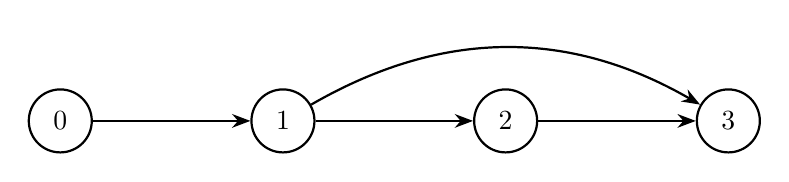
\begin{tikzpicture}[
            node distance=2cm,
            every node/.style={circle, draw, minimum size=8mm},
            every path/.style={->, thick, >=Stealth}
          ]

          % Nodes in a straight line
          \node (0) {0};
          \node[right=of 0] (1) {1};
          \node[right=of 1] (2) {2};
          \node[right=of 2] (3) {3};

          % Edges
          \draw (0) -- (1);
          \draw (1) -- (2);
          \draw[bend left=30] (1) to (3); % Curved edge from 1 to 3
          \draw (2) -- (3);

        \end{tikzpicture}

        where $a = 1$ and $b = 2$
      \end{mdframed}
      \end{mdframed}
      

      \item  Consider the following algorithm for computing the dominator
      relation for a CFG with nodes $\{1,2,\dots,n\}$:

      {\centering
      \begin{minipage}{.9\linewidth}
        \begin{algorithm}[H]
          \SetAlgoRefName{1}
          \SetKwData{domKw}{DOM}
          \SetKw{returnKw}{return}
          \DontPrintSemicolon
          \KwIn{Directed graph $G$ with nodes $\{1,2,\dots,n\}$, sequence $L$ of graph nodes}

          \KwOut{Dominators $\domKw$ }
       
          \ForEach{$v \in \{1, 2, \dots, n\}$} {
            $\domKw[v] \coloneqq \{1, 2, \dots, n\}$
          }
          \ForEach{$v \in L$} {
            $\domKw[v] \coloneqq \big( \bigcap_{p \in pred(v)} \domKw[p] \big) \cup \{v\}$\label{li:update}
          }
          \returnKw{$\domKw$}
        \caption{ComputeDominator($G$, $L$)}
        \label{alg:dom}
        \end{algorithm}
      \end{minipage}
      \par
      }

      The above algorithm is similar to the iterative dominator algorithm
      discussed in class; in particular, the update to $DOM[v]$ on
      line~\ref{li:update} is the same. However, instead of iterating over all
      the nodes until fixpoint, the above algorithm merely traverses the nodes
      in $L$ once. It should be clear that the correctness and performance of
      the above algorithm depends entirely on the list $L$ passed as input. We
      refer to a sequence $L$ that can be used by Algorithm~\ref{alg:dom} to
      correctly compute dominators for the graph $G$ as a \emph{dominator
      sequence} for $G$.

      \begin{figure}[t]
        \centering
        \begin{subfigure}[b]{0.50\linewidth}
          \centering
          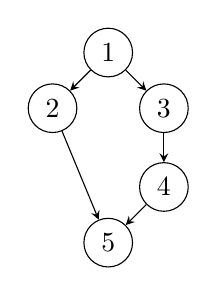
\begin{tikzpicture}[auto,node distance=1cm]
          \tikzstyle{every node} = [circle, draw]
          \node (1) {1};
          \node [below left of=1] (2) {2};
          \node [below right of=1] (3) {3};
          \node [below of=3] (4) {4};
          \node [below left of=4] (5) {5};
          
          \path (1) edge[cfgedge] (2);
          \path (1) edge[cfgedge] (3);
          \path (2) edge[cfgedge] (5);
          \path (3) edge [cfgedge](4);
          \path (4) edge[cfgedge] (5);
          \end{tikzpicture}
        \caption{Graph $G_2$}
        \label{fig:graph2}
        \end{subfigure}
        %
        \begin{subfigure}[b]{0.40\linewidth}
          \centering
          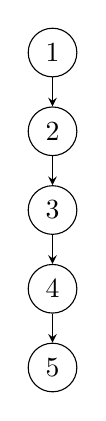
\begin{tikzpicture}[auto,node distance=1cm]
          \tikzstyle{every node} = [circle, draw]
          \node  (3) {1};
          \node [below  of=3] (4) {2};
          \node [below  of=4] (5) {3};
          \node [below of=5] (6) {4};
          \node [below of=6] (7) {5};
          
          \path (3) edge[cfgedge] (4);
          \path (4) edge[cfgedge] (5);
          \path (5) edge [cfgedge](6);
          \path (6) edge[cfgedge] (7);
          \end{tikzpicture}
        \caption{Graph $G_3$}
        \label{fig:graph3}
        \end{subfigure}
      \caption{}
      \end{figure}

      For the graph $G_2$ (Figure~\ref{fig:graph2}), the sequence $[1,2,3,4,5]$
      is a dominator sequence and so is the sequence $[1,3,2,4,5]$.
      The sequence $[1, 2,3,5,4]$ is NOT a dominator sequence, while
      the sequence $[1,2,3,5,4,5]$ is a dominator sequence. 
      
      \begin{enumerate} 
        \item (4 points) List the \emph{shortest} dominator sequence for the
        graph $G$ in Figure~\ref{fig:graph1}.
        \begin{mdframed}
          %% TODO
          $L = [1, 2, 3, 4, 5, 6, 7, 8]$
        \end{mdframed}

        \item (4 points) List the \emph{shortest} dominator sequence for the
        graph $G_3$ in Figure~\ref{fig:graph3}.
        \begin{mdframed}
          %% TODO
          $L = [1, 2, 3, 4]$
        \end{mdframed}

        \item (10 points) State whether the following statement is \textbf{True}
        or \textbf{False}: 

          \emph{The length of the shortest dominator sequence for any flow graph
          $G$ with $N$ nodes is at most $N$.}

        If \textbf{True}, provide a proof. If \textbf{False}, provide a
        counter-example in the form of the flow graph $G$ and the shortest
        dominator sequence $L$.
        \begin{mdframed}
        \textbf{True}

From our previous proof, we know that a Control Flow Graph (CFG) $G$ and $G-$ share the same dominator relationships, where $G-$ is the CFG $G$ but with all retreating edges removed. Therefore, for the purpose of this proof, we assume that every CFG $G$ has an equivalent CFG $G-$ because any CFG can be translated into $G-$ without affecting the structure of its dominator tree.

   As shown above in the pseudocode for ComputesDominator, the dominator algorithm computes the correct dominator sets in a single pass, provided that every time we examine a node, it's predecessors already have correct dominator information. This is seen in the line 4 where we intersect the dominator sets for all $p$ predecessors. It is clear from this line that if the dominator sets for all the predecessors is correct, then the dominator set for the successor will be correct, since all the predecessors will have the correct information.

    We can exploit this to generate a valid dominator sequence. Since $G-$ is just $G$ but without any of the retreating edges, we can say it is acyclic—i.e., a node \( x \) cannot have a descendant \( y \) that is also a predecessor of \( x \). In other words, there are no cycles.

    Thus, we want to schedule the nodes so that whenever a node is processed, all of its predecessors have already been processed and have valid dominator information. This scheduling can be achieved using a dependency graph:

    \begin{itemize}
      \item For each node \( n \) in $G-$:
      \begin{itemize}
        \item For each predecessor \( p \) of \( n \), add a directed edge from \( n \) to \( p \) in the dependency graph.
      \end{itemize}
    \end{itemize}

    After constructing this dependency graph, we perform a topological sort. The resulting ordering ensures that every node appears after its predecessors, guaranteeing that when we compute the dominators of a node, all necessary data is already available.

    This algorithm is correct because it explicitly encodes the dependency of each node on its predecessors. The topological sort then provides a valid sequence for dominator computation.

    Since the dependency graph contains \( N \) nodes, the topological sort will always yield a sequence of length \( N \). However, in practice, we can sometimes shorten this sequence by omitting nodes whose dominator sets remain at the initialized value (i.e., all nodes in the graph). These nodes don't need to appear in the sequence.

    Therefore, we have shown that the dominator sequence of any CFG with \( N \) nodes is of length at most \( N \).

      
      %% \textbf{False} PROVIDE COUNTER-EXAMPLE
    \end{mdframed}
      \end{enumerate}

      \item State whether the following statements are \textbf{True} or
      \textbf{False}:
      \begin{enumerate}
        \item (3 points) \emph{For all nodes $x, y$ in a CFG, if node $x$ is
        control dependent on node $y$, \\
        then there is a path from $y$ to $x$ in the CFG.}

        If \textbf{True}, provide a proof.
        If \textbf{False}, provide a counter-example in the form of the flow
        graph $G$ and and nodes $x$ and $y$.
        \begin{mdframed}
          \textbf{True}

          \textbf{Proof:}

          Assume that node $x$ is control dependent on node $y$. By definition of control dependence, the following two conditions hold:

          \begin{enumerate}
            \item node $x$ postdominates some successor $s$ of node $y$, and
            \item node $x$ does not strictly postdominate node $y$.
          \end{enumerate}

          Condition (1) implies that every path from $s$ to the exit must pass through $x$. In particular, this means that there exists a path from $s$ to $x$ in the CFG.

          Since $s$ is a successor of $y$, there is a direct edge from $y$ to $s$. Therefore, we can construct a path from $y$ to $x$ by first following the edge from $y$ to $s$, and then following the path from $s$ to $x$.

          Thus, there exists a path from node $y$ to node $x$ in the CFG.
        \end{mdframed}
      
        \item (3 points)
        \emph{For all nodes $x, y$ in a CFG, if node $x$ is control dependent on
        node $y$, then node $y$ is NOT control dependent on node $x$.}

        If \textbf{True}, provide a proof.
        If \textbf{False}, provide a counter-example in the form of the flow
        graph $G$ and and nodes $x$ and $y$.
        \begin{mdframed}
          %% TODO
          %% \textbf{True} PROVIDE PROOF
          \textbf{False}

          \textbf{Counter Example:}
          \begin{mdframed}
            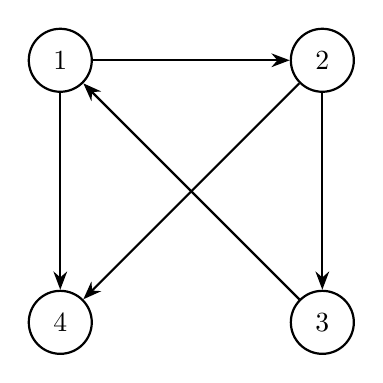
\begin{tikzpicture}[
              node distance=2.5cm and 2.5cm,
              every node/.style={circle, draw, minimum size=8mm},
              every path/.style={->, thick, >=Stealth}
            ]

            % Nodes
            \node (1) {1};
            \node[right=of 1] (2) {2};
            \node[below=of 2] (3) {3};
            \node[below=of 1] (4) {4};

            % Edges
            \draw (1) -- (2);
            \draw (1) -- (4);
            \draw (2) -- (3);
            \draw (2) -- (4);
            \draw (3) -- (1);

            \end{tikzpicture}

            where $x = 2$ and $y = 1$ and node $1$ is the entry node and node $4$ is the exit node
          \end{mdframed}
        \end{mdframed}
      
        \item (3 points) \emph{For all nodes $x, y, z$ in a CFG, if node $x$ is
        control dependent on node~$y$, and node $y$ is control dependent on
        node~$z$, then node $x$ is control dependent on node $z$.}

        If \textbf{True}, provide a proof. If \textbf{False}, provide a
        counter-example in the form of the flow graph $G$ and and nodes $x$,
        $y$, and $z$.
        \begin{mdframed}
          %% TODO
          %% \textbf{True} PROVIDE PROOF
          \textbf{False}

          \textbf{Counter Example:}
          \begin{mdframed}
            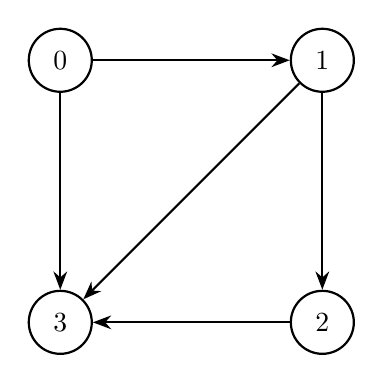
\begin{tikzpicture}[
    node distance=2.5cm and 2.5cm,
    every node/.style={circle, draw, minimum size=8mm},
    every path/.style={->, thick, >=Stealth}
  ]

  % Nodes
  \node (0) {0};
  \node[right=of 0] (1) {1};
  \node[below=of 1] (2) {2};
  \node[below=of 0] (3) {3};

  % Edges for 0
  \draw (0) -- (1);
  \draw (0) -- (3);

  % Edges for 1
  \draw (1) -- (2);
  \draw (1) -- (3);

  % Edges for 2
  \draw (2) -- (3);

\end{tikzpicture}
          where $x = 2$ and $y = 1$ and $z = 0$ and node $0$ is the entry node and node $3$ is the exit node
          \end{mdframed}
        \end{mdframed}
      \end{enumerate}
      
    \end{enumerate}
    
    \end{document}
